\documentclass[12pt,a4paper]{ctexart}

\title{\zihao{-2}关于代数基本定理的猜想与研究}
\author{高一(13)班\ \ \ 郑庭昊}

\setlength{\parskip}{0em}
\usepackage{xeCJK,amsmath,mathtools,amssymb,geometry,wrapfig,graphicx,empheq,pifont}
\renewcommand{\baselinestretch}{1.73}
\geometry{left=2.5cm,right=2.5cm,bottom=2cm,top=2.7cm}
\usepackage{tikz}
\usepackage{xcolor}
\newcounter{exam}[section]
\setcounter{exam}{0}
\renewcommand{\thefootnote}{*}

\begin{document}
\maketitle
\pagenumbering{roman}
\tableofcontents
\newpage
\pagenumbering{arabic}


\setlength{\abovedisplayskip}{3pt}
\setlength{\belowdisplayskip}{3pt}

\section{研究背景}
 {
  \zihao{-3}\fangsong 在代数发展史上的很长一段时期内,解一元多项式方程一直是人们研究的一
  个中心问题.早在古巴比伦时期人们就会解一元二次方程. 16世纪上半叶,数
  学家们得到了一元三次方程,一元四次方程的解法.此后,数学
  家们转向求解一元五次及五次以上的方程.他们想弄清楚以下问题:一般的一元
  多项式方程有没有根?如果有根,根的个数是多少?是否存在求根公式? 在数学的
  不断发展下, 这个问题早已经被解决.《数学必修\ 第二册》第81页对这个问题
  做了基本的介绍, 并给我们留下了习题. 对此我们继续展开研究.

 }

\section{研究目标}

 {
  \zihao{-3}\fangsong 通过研究性学习进一步了解代数学, 增强数学素养, 提高数学能力和兴趣. 尝试证明代数基本定理及其推论
  , 研究一元多项式方程根与系数的关系, 并在实际问题中应用它们.

 }

\section{研究成果}

\subsection{代数基本定理的演化和证明史}

{\zihao{-3}\fangsong 从算数到代数,是人类抽象认识世界能力一次跨越式的发展.我们可以从剥离了具体对象特征来用统一的自然数给集合计数以外,
    能够继续再把这具体的数量抽象成用字母来表示的数,研究的是其作为任何数的统一的特征和性质,
    而不再关心任何一个具体的数.

    而当我们引入代数,再引入方程,自然而然地,我们就遇到了诸如 4 + 多少 = 2 的问题,
    于是产生了负数的概念.以及那最经典的故事: 当我们在求解$x^2 = -1$的时候,
    对$x$的解的需求使我们引入了复数. 这些定义看起来越来越不切实际,
    但是随着数学大厦的不断拓展, 我们找到了其新的物理意义和应用点.

    而整个代数大厦的根基,还数代数基本定理.

    17 世纪的代数方程论开始于方程根的数目究竟有多少的问题.
    吉罗拉莫·卡尔达诺第一个意识到三次方程可能有三个根,
    四次方程可能有四个根等.但他只考虑了正根,没有考虑负根.

    1629年荷兰数学家阿尔伯特∙吉拉德在“代数的新发明”一书中断言,如果把虚根考虑在内,
    并按重数计算重根的数目,则$݊n$次代数方程有$݊n$个根.吉拉德首次将负数与正数等量齐观并承认复根,
    虽未能给出证明,但克服了大多数数学家不愿将复数根视为合理的情况.

    1637 年勒内·笛卡尔在他的“几何学”第三卷中推测每个方程根的数目等于未知数的维数,与吉拉德的说法类似,
    但是对笛卡尔来说, 虚根从来不对应任何实数,他摒弃了复根.

    18 世纪初,约翰·伯努利和戈特弗里德·威廉·莱布尼茨的工作构成了代数基本定理史的起点,
    开启了一段围绕实系数多项式能分解成线性因式的乘积为主题的工作.

    对于方程根的存在性问题的普遍关注是在十八世纪,代数基本定理的第一次证明通常归功于法国数学家让·勒朗·达朗贝尔,
    他在1746年详细阐述了此定理,并于1748年出版.后续的几年里, 许多数学家给出了该定理的其他证明方法, 但仍有缺陷.

    代数基本定理的第一个严格证明通常认为是高斯给出的.高斯一生为此定理提供 4次证明:1799 年的第一次证明作为博士
    论文发表于赫尔姆施泰特大学,在以后的1815 年、1816 年、1849年分别给出代数基本定理的另外三个证明.

    据说,关于代数学基本定理的证明,现有200多种证法.

}
\fangsong
\subsection{复数的表示\ \ \ 复变函数}

一般的一元多项式方程有没有根? 如果有根,根的个数是多少? 是否存在求根公式? 早在 16 世纪以前,
数学家们就得到了一元二次方程, 一元三次方程, 一元四次方程的求根公式, 但五次及以上的方程就没有
求根公式了.那我们如何保证根的存在性呢?

代数基本定理正好回答了这个问题.

\subparagraph{代数基本定理} \textbf{\heiti 任何一元$n (n \in \mathbb{N^*} )$次复系数多项式方程$f(x) = 0$
    在复数域上至少有一根.}\\

这个定理的证明在一般的高中教材, 甚至在大学的高等代数教材里, 都只是一带而过.
那我们是否在高中阶段就没办法理解和掌握代数基本定理的证明了呢?

在证明这个定理之前, 我们先要了解一些预备知识. 第一个是复数的三角表示和指数表示.
《数学必修 第二册》教材第7.3节对此进行了一些介绍,
不过是选学的内容.

\subsubsection{复数的三角表示与指数表示}

\begin{wrapfigure}{r}{5cm}
    \flushright
    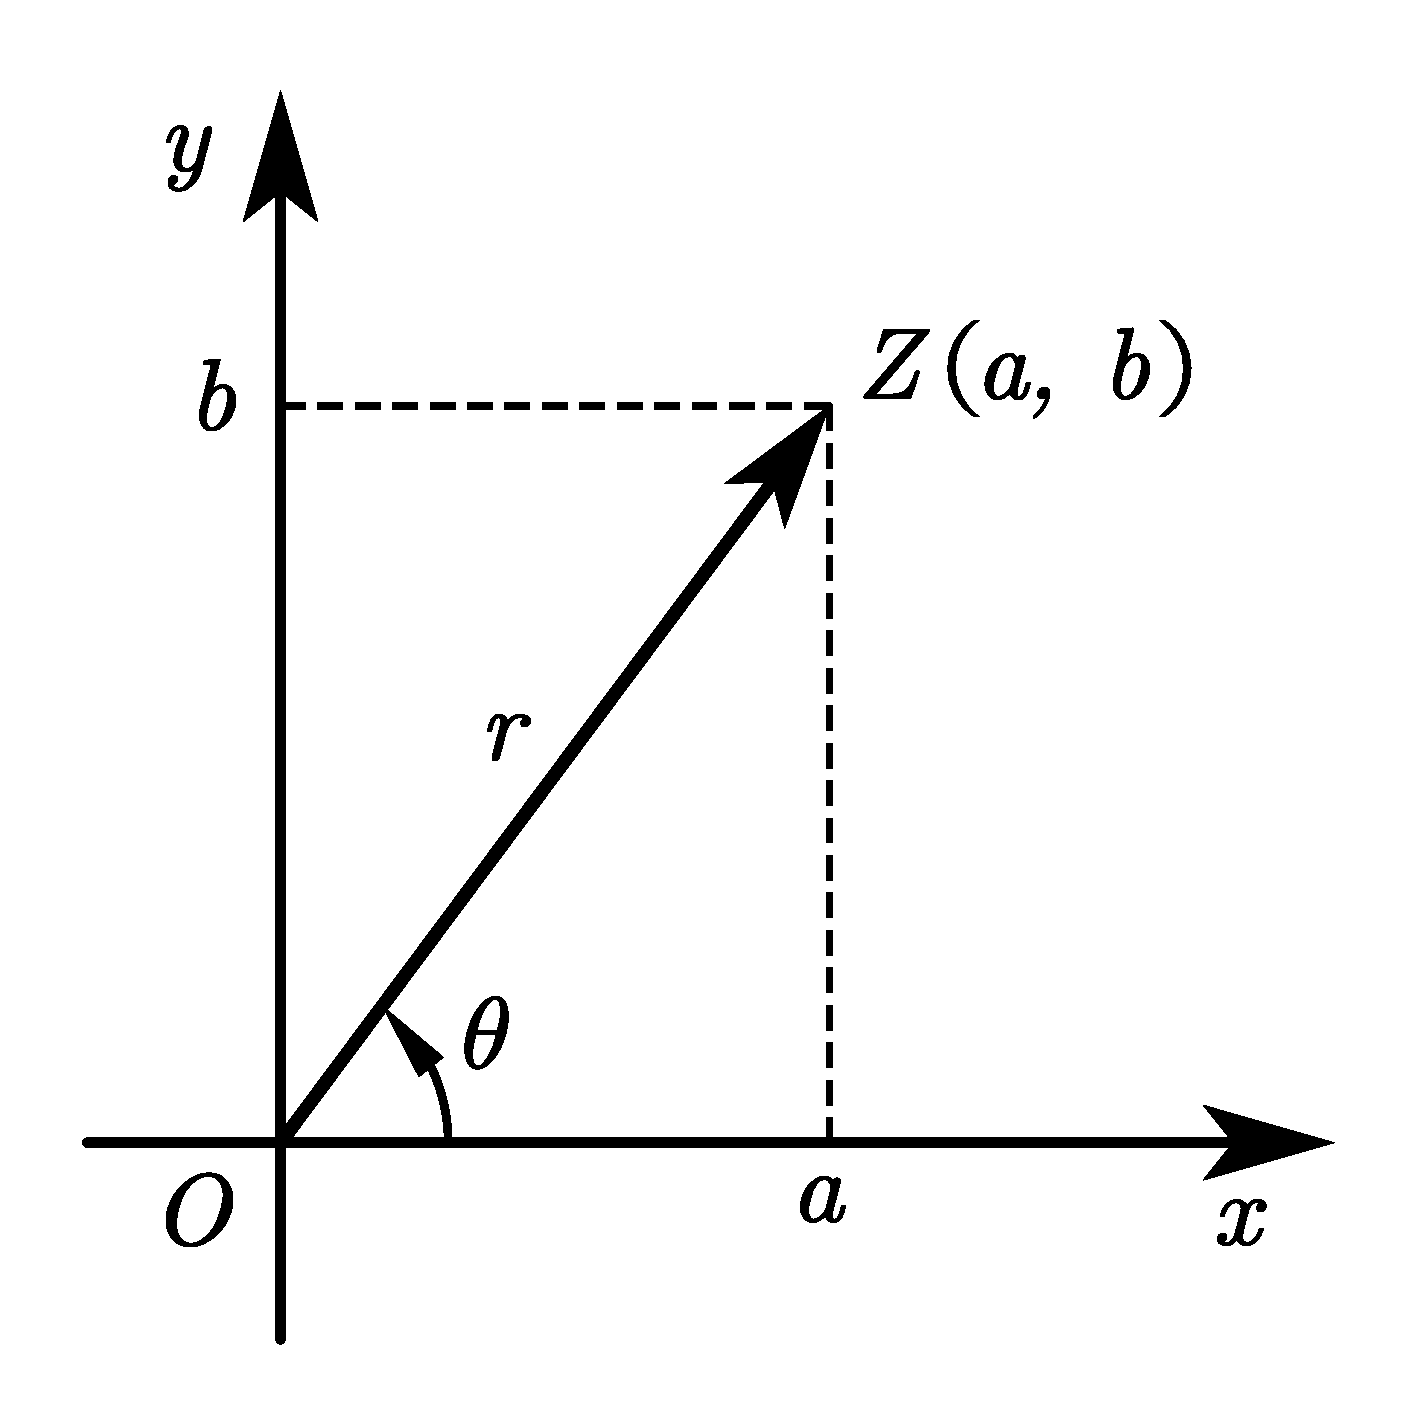
\includegraphics[width=0.3\textwidth]{Untitled.pdf}
    \label{fig5}
\end{wrapfigure}

把一个复数$z = a+b\mathrm{i}$在复平面内表示为
向量$\overrightarrow{OZ}$, 如图所示. 并记
$$r = \left\lvert z \right\rvert = \left\lvert a + b\mathrm{i} \right\rvert .$$
由此可知
\begin{equation*}
    \begin{cases*}
        a = r\cos \theta, \\
        b = r\sin \theta.
    \end{cases*}
\end{equation*}
因此
\begin{align*}
    z = a + b\mathrm{i} & = r\cos \theta + \mathrm{i}r \cos \theta  \\
                        & = r(\cos \theta + \mathrm{i}\sin \theta).
\end{align*}

我们把$r(\cos \theta + i\sin \theta)$叫做\textbf{复数$z$的三角表示}.其中
向量$\overrightarrow{OZ}$与实轴的夹角$\theta$叫做复数$z$的\textbf{辐角}.由任意角的知识
可知, 一个复数的辐角有无数多个值, 我们规定在$[0, 2\pi]$范围内的辐角$\theta$的值为
\textbf{辐角的主值}, 记作$\arg z$.

除此之外, 我们定义$\mathrm{e}^{\mathrm{i}\theta} = \cos \theta + i\sin \theta$, 称为欧拉公式,
其中$\mathrm{i}$是虚数单位, $\mathrm{e}$是自然对数的底数. 因此
$$z = r(\cos \theta + \mathrm{i}\sin \theta) = r\mathrm{e}^{\mathrm{i}\theta},$$称为复数$z$的\textbf{指数表示}.由定义可知,
$$|r\mathrm{e}^{\mathrm{i}\theta}| = r.$$

\subsubsection{复变函数}

了解完复数的表示, 我们再来了解一下复变函数.

设$A$是一个复数集, 如果对$A$中的任一复数$z$,
通过一个确定的规则有一个或若干个复数$w$与之对应,就说在复数集$A$上定义了一个\textbf{复变函数},
记作$$w = f(z), z \in A.$$

复变函数$w = f(z)$的零点就是方程$f(z) = 0$的复数根.

\subsection{代数基本定理的简单证明}

要想证明代数基本定理, 我们还需要了解两个命题.

\begin{enumerate}
    \item 多项式复变函数的模在复平面上连续, 而连续函数在闭圆盘上一定有最大和最小值.\label{1}
    \item 多项式复变函数当自变量趋于无穷大时, 函数值的模也趋于无穷大.\label{2}
\end{enumerate}

\ref{1} 的证明需要用到高等数学知识,故略去;而 \ref{2} 是显然的.

由 \ref{1} 和 \ref{2} 可得多项式复变函数在整个复平面上一定有最小值.
即使没有学过高等数学知识, 只要承认 \ref{1} 的正确性,
也可以理解证明.\newpage
\setlength{\abovedisplayskip}{3pt}
\setlength{\belowdisplayskip}{3pt}

有了复变函数的概念, 我们可以把代数基本定理转化为符号语言.

\setlength{\abovedisplayskip}{10pt}
\setlength{\belowdisplayskip}{10pt}

\subparagraph{代数基本定理} \textbf{\heiti 对任意的$n$次多项式复变函数
    $$f(z) = \sum_{i = 0}^{n} c_i z^i = c_0 + c_1z + c_2z^2 +\cdots+ c_nz^n, c_n \neq 0$$
    都存在$z_0 \in \mathbb{C}$, 使$f(z_0) = 0$.}

\textbf{证明}\ \ \  用反证法. 假设$f(z)$没有零点. 根据 \ref{1}, $|f(z)|$在复平面上连续, 并且
$|f(z)|$一定有最小值$r_0 > 0$.

不妨设在$z_0$处取得最小值$|f(z_0)| = r_0$, 而$f(z_0) = r_0 \mathrm{e}^{\mathrm{i}\theta_0}$
(其中$\theta_0 = \arg(f(z_0))$). 把$z$替换为$z + z_0$, 可得
$$
    f(z+z_0)          = r_0 \mathrm{e}^{\mathrm{i}\theta_0} + c_k^{\prime} z^k + c_{k+1}^{\prime} z^{k+1}\cdots + c_n^{\prime}z^n $$ $$
    \Rightarrow f(z)  = r_0 \mathrm{e}^{\mathrm{i}\theta_0} + c_k^{\prime} (z-z_0)^{k} + c_{k+1}^{\prime} (z-z_0)^{k+1} + \cdots + c_n^{\prime} (z-z_0)^n.
$$
其中$r_0 \mathrm{e}^{\mathrm{i}\theta_0}$
是常数项, $c_k^{\prime} \neq 0\ (k\in \mathbb{N}^*, k<n)$是除常数项外最低次非零项的系数\footnote{由泰勒展开可知, 变量替换后的多项式系数除最高次系数与原系数相同, 其它项系数与原系数不一定相同. 事实上, $c^{\prime}_n = c_n$, 为了便于理解, 这里不写为$c_n$.}.

在$z = z_0$附近, $f(z)$和$g(z) = r_0 \mathrm{e}^{\mathrm{i}\theta_0} + c_k^{\prime} (z-z_0)^k$
的值很接近.事实上, 当$0 < |z-z_0| \leqslant 1$时, $0 < |z-z_0|^i \leqslant 1$ $(i = k, k+1,\cdots,n-k+1)$,
从而
\setlength{\abovedisplayskip}{15pt}
\setlength{\belowdisplayskip}{5pt}
\begin{align*}
    \left\lvert \frac{f(z)-g(z)}{(z-z_0)^{k+1}} \right\rvert & = \left\lvert \frac{c_{k+1}^{\prime} (z-z_0)^{k+1} + c_{k+2}^{\prime} (z-z_0)^{k+2} + \cdots +c_{n}^{\prime} (z-z_0)^{n}}{(z-z_0)^{k+1}}\right\rvert \\
                                                             & \leqslant \left\lvert c^{\prime}_{k+1} + c^{\prime}_{k+2} + \cdots + c_n^{\prime} \right\rvert                                                       \\
                                                             & \leqslant \left\lvert c_{k+1}^{\prime} \right\rvert + \left\lvert c_{k+2}^{\prime} \right\rvert + \cdots + \left\lvert c_{n}^{\prime} \right\rvert.
\end{align*}

\setlength{\abovedisplayskip}{3pt}
\setlength{\belowdisplayskip}{3pt}

我们记$M = \left\lvert c_{k+1}^{\prime} \right\rvert + \left\lvert c_{k+2}^{\prime} \right\rvert + \cdots + \left\lvert c_{n}^{\prime} \right\rvert$
,可以得到
\begin{align*}
    \left\lvert f(z)-g(z) \right\rvert \leqslant M |z-z_0|^{k+1}.
\end{align*}
由不等式的知识可得$|f(z)|-|g(z)|\leqslant |f(z)-g(z)|$, 从而
$$\left\lvert f(z) \right\rvert \leqslant |g(z)| + M|z-z_0|^{k+1}.$$

设$r\mathrm{e}^{\mathrm{i}\theta} = z-z_0$,
其中$0 < r \leqslant 1$, 由此可得
\begin{align*}
    f(z) & \leqslant |r_0 \mathrm{e}^{\mathrm{i}\theta_0} + c_k^{\prime} (r\mathrm{e}^{\mathrm{i}\theta})^k| + M|r\mathrm{e}^{\mathrm{i}\theta}|^{k+1} \\
         & = |r_0 \mathrm{e}^{\mathrm{i}\theta_0} + c_k^{\prime} r^{k}\mathrm{e}^{\mathrm{i} k\theta}| + Mr^{k+1}.
\end{align*}
为了使$|r_0 \mathrm{e}^{\mathrm{i}\theta_0} + c_k^{\prime} r^{k}\mathrm{e}^{\mathrm{i} k\theta}|$
最小, 我们取$\theta$使得$\mathrm{e}^{\mathrm{i}k\theta} = -1$, 于是
\setlength{\abovedisplayskip}{3pt}
\setlength{\belowdisplayskip}{10pt}
\begin{align*}
    f(z) & \leqslant |r_0\mathrm{e}^{\mathrm{i}\theta_0} - c_k^{\prime}r^k| + Mr^{k+1}   \\
         & \leqslant |r_0\mathrm{e}^{\mathrm{i}\theta_0}| - |c_k^{\prime}r^k| + Mr^{k+1} \\
         & = r_0 - |c_k^{\prime}|r^k + Mr^{k+1}                                          \\
         & = r_0 - r_k(|c^{\prime}_k| - Mr).
\end{align*}

当$|c^{\prime}_k| - Mr > 0$时, 即$0 < r < \displaystyle\frac{|c^{\prime}_k|}{M}$时,
$|f(z)| < r_0$, 这
与$r_0$的定义矛盾, 故假设不成立.即$|f(z)|$的最小值一定是0, 为$f(z)$的零点.
$\hfill\square $

\subsection{代数基本定理的推论}

由代数基本定理知, 任意一个一元一次复系数多项式
$$w_i(z) = a_iz + b_i, a, b\in \mathbb{C}, a_i \neq 0 $$一定有1个根,
我们把$n$个这样的多项式相乘, 并记
\setlength{\abovedisplayskip}{10pt}
\setlength{\belowdisplayskip}{15pt}
$$g(z) = c\prod_{i=1}^{n}w_i(z) = cw_1(z)w_2(z)\cdots w_n(z), c\neq 0.\ \footnote{$\prod$是求积符号.\ $\displaystyle\prod_{i=1}^{n}x_i = x_1x_2\cdots x_n.$}$$


\setlength{\abovedisplayskip}{3pt}
\setlength{\belowdisplayskip}{3pt}
显然, 每一个$z_i$使$w_i(z_i) = 0$, 都是$g(z) = 0$的一个根. 所以$n$次复系数多项式方程
$g(z) = 0$有$n$个根(重根按重数计).因此, 我们有如下推论.

\subparagraph{推论} \textbf{\heiti 一元$n (n\in \mathbb{N}^* )$次多项式方程有$n$个复数根(重根按重数计).}\\

我们举几个例子.

一元一次方程$x-1=0$有1个根$x = 1$.

一元二次方程$x^2-1=0$有2个实数根$x_1 = 1, x_2 = -1$;
一元二次方程$x^2+1=0$有2个虚数根 $x_1 = \mathrm{i}, x_2 = -\mathrm{i}.$
它们都有2个复数根.

同理, 一元三次方程$x^3-1 = 0$应该有3个复数根. 我们显然能看出来其中一个根是$x = 1$,
那另外两个根呢?

利用立方差公式, 原方程可化为$$(x-1)(x^2 + x + 1) = 0,$$
于是$$x - 1 = 0, \text{\ 或\ } x^2 + x + 1 = 0.$$

$x^2 + x + 1 = 0$这个方程我们会解, 它的两个根分别是
$\displaystyle\frac{-1+\sqrt{3}\mathrm{i}}{2}$和
$\displaystyle\frac{-1-\sqrt{3}\mathrm{i}}{2}$. 因此,
$x^3-1 = 0$的3个复数根分别为
\setlength{\abovedisplayskip}{10pt}
\setlength{\belowdisplayskip}{10pt}
$$x_1 = 1, x_2 = \frac{-1+\sqrt{3}\mathrm{i}}{2}, x_3 = \frac{-1-\sqrt{3}\mathrm{i}}{2}.$$

我们再来看一元四次方程$x^4-1 = 0$. 我们能直接看出它的4个根
\setlength{\abovedisplayskip}{3pt}
\setlength{\belowdisplayskip}{3pt}
$$x_1 = 1, x_2 = -1, x_3 = \mathrm{i}, x_4 = -\mathrm{i}.$$

通过以上四个例子可以看出, 一元多项式方程复数根的个数确实和它的次数相等.

\subsection{一元多项式方程根与系数的关系}

从代数基本定理的推论出发, 我们来研究一元多项式方程的根与系数之间的关系.

设一元二次方程$$a_2x^2 + a_1x + a_0 = 0\ (a_2 \neq 0).$$
根据代数基本定理的推论, 它在复数集$\mathbb{C}$内应该有2个根, 不妨设它们分别为
$x_1, x_2$, 容易得到
\setlength{\abovedisplayskip}{10pt}
\setlength{\belowdisplayskip}{10pt}
$$\begin{cases*}
        x_1 + x_2 = -\displaystyle\frac{a_1}{a_2}, \\
        x_1x_2 = \displaystyle\frac{a_0}{a_2}.
    \end{cases*}$$
\setlength{\abovedisplayskip}{3pt}
\setlength{\belowdisplayskip}{3pt}

同理, 设一元三次方程$$a_3x^3 + a_2x^2 + a_1x + a_0 = 0\ (a_3 \neq 0)$$
在复数集$\mathbb{C}$内的3个根为$x_1, x_2, x_3$, 教材已经告诉我们
\setlength{\abovedisplayskip}{10pt}
\setlength{\belowdisplayskip}{10pt}
$$\begin{cases*}
        x_1 + x_2 + x_3 = -\displaystyle\frac{a_2}{a_3},         \\
        x_1x_2 + x_1x_3 + x_2x_3 = \displaystyle\frac{a_1}{a_3}, \\
        x_1x_2x_3 = -\displaystyle\frac{a_0}{a_3}.
    \end{cases*}$$
下面我们来看一元四次方程.
\setlength{\abovedisplayskip}{3pt}
\setlength{\belowdisplayskip}{3pt}

设一元四次方程
\begin{equation}
    a_4x^4 + a_3x^3 + a_2x^2 + a_1x + a_0\ (a_4 \neq 0)
    \label{5}
\end{equation}
在复数集$\mathbb{C}$内的4个根为$x_1, x_2, x_3, x_4$, 则方程 \eqref{5}
可变形为
$$a_4(x - x_1)(x - x_2)(x - x_3)(x - x_4) = 0,$$
展开得
\begin{equation}
    \begin{split}
        a_4x^4 - a_4(x_1 + x_2 + x_3 + x_4)x^3 + a_4(x_1x_2 + x_1x_3 + x_1x_4 + x_2x_3 + x_2x_4 + x_3x_4)x^2 \\- a_4(x_1x_2x_3 + x_1x_2x_4 + x_1x_3x_4 + x_2x_3x_4)x + a_4x_1x_2x_3x_4.
        \label{6}
    \end{split}
\end{equation}
比较 \eqref{5}\eqref{6} 可以得到
\setlength{\abovedisplayskip}{10pt}
\setlength{\belowdisplayskip}{10pt}
$$\begin{cases*}
        x_1 + x_2 + x_3 + x_4 = -\displaystyle\frac{a_3}{a_4},                              \\
        x_1x_2 + x_1x_3 + x_1x_4 + x_2x_3 + x_2x_4 + x_3x_4 = \displaystyle\frac{a_2}{a_4}, \\
        x_1x_2x_3 + x_1x_2x_4 + x_1x_3x_4 + x_2x_3x_4 = -\displaystyle\frac{a_1}{a_4},      \\
        x_1x_2x_3x_4 = \displaystyle\frac{a_0}{a_4}.
    \end{cases*}$$

类似地, 设一元五次方程
\setlength{\abovedisplayskip}{3pt}
\setlength{\belowdisplayskip}{3pt}
$$a_5x^5 + a_4x^4 + a_3x^3 + a_2x^2 + a_1x + a_0 = 0\ (a_5 \neq 0)$$
在复数集$\mathbb{C}$内的5个根为$x_1, x_2, x_3, x_4, x_5$, 可以得到
\setlength{\abovedisplayskip}{10pt}
\setlength{\belowdisplayskip}{10pt}
$$\begin{cases*}
        x_1 + x_2 + x_3 + x_4 + x_5 = -\displaystyle\frac{a_4}{a_5},                                                                                   \\
        x_1x_2 + x_1x_3 + x_1x_4 + x_1x_5 + x_2x_3 + x_2x_4 + x_2x_5 + x_3x_4 + x_3x_5 + x_4x_5 = \displaystyle\frac{a_3}{a_5},                        \\
        x_1x_2x_3 + x_1x_2x_4 + x_1x_2x_5 + x_1x_3x_4 + x_1x_3x_5 + x_1x_4x_5 + x_2x_3x_4                                                              \\
        \ \ \ \ \ \ \ \ \ \ \ \ \ \ \ \ \ \ \ \ \ \ \ \ \ \ \ \ \ \ \ \ \ \ \ \ \ + x_2x_3x_5 + x_2x_4x_5 + x_3x_4x_5 = -\displaystyle\frac{a_2}{a_5}, \\
        x_1x_2x_3x_4 + x_1x_2x_3x_5 + x_1x_2x_4x_5 + x_1x_3x_4x_5 + x_2x_3x_4x_5 = \displaystyle\frac{a_1}{a_5},                                       \\
        x_1x_2x_3x_4x_5 = -\displaystyle\frac{a_0}{a_5}.
    \end{cases*}$$
至此, 我们应该已经找到规律了.
\setlength{\abovedisplayskip}{3pt}
\setlength{\belowdisplayskip}{3pt}

一般地, 设一元$n(n \in \mathbb{N}^*)$次多项式方程
$$a_0 + a_1x + a_2x^2 + \cdots + a_nx^n = 0\ (a_n \neq 0)$$
的$n$个根分别为$x_1, x_2, \cdots, x_n$,则有
$$x_1 + x_2 + \cdots + x_n = -\frac{a_{n-1}}{a_n}.$$


从这$n$个根中取出$m(m\in \mathbb{N}^*, m\leqslant n)$个求积, 最多能得到$C_n^m$种因式.把这$C_n^m$个因式求和,
得到
\begin{equation*}
    \sum^{n-m+1}_{i_1 = 1}\sum^{n-m+2}_{i_2 = i_1 + 1} \cdots \sum^{n}_{i_m = i_{m-1} + 1}\prod_{j = 1}^{m}x_{i_{j}}:=S.\ \footnote{$f(x):=M$表示把式子$f(x)$记为$M$.}
\end{equation*}
则有
$$
    S = \begin{cases*}
        -\displaystyle\frac{a_{n-m}}{a_n},  & $m$\text{\ 为奇数}, \\
        \ \displaystyle\frac{a_{n-m}}{a_n}, & $m$\text{\ 为偶数}.
    \end{cases*}
$$

特别地, 当$m = n$时, $$S^{\prime} = x_1x_2\cdots x_n.$$
于是有
$$
    x_1x_2\cdots x_n = \begin{cases*}
        -\displaystyle\frac{a_{0}}{a_n},  & $m$\text{\ 为奇数}, \\
        \ \displaystyle\frac{a_{0}}{a_n}, & $m$\text{\ 为偶数}.
    \end{cases*}
$$\\

这就是一元$n$次多项式方程的根与系数之间的关系, 它对实系数和复系数都适用, 即前述的$a_i \in \mathbb{C}\ (i = 1, 2, \cdots, n).$

以上就是本次研究性学习的全部内容.

\end{document}